% Content for Chapter 5, Section 5.4 — pulled in by chapters/05-system-design.tex
\subsection{مكوّنات الخدمة}

% CH2-REF: originally "(\en{Clean Architecture}) الموصوف في القسم~\ref{subsec:clean-architecture}،" — restore with chapter 2.
اتُّبع في تصميم هذه الخدمة، كما في بقية خدمات \en{.NET}، نمطُ المعمارية النظيفة (\en{Clean Architecture})، بأربع طبقات متّحدة المركز تتّجه التبعيات فيها نحو الداخل. ويعرض الشكل~\ref{fig:comp-01} مكوّنات الخدمة موزّعةً على هذه الطبقات مع روابطها الخارجية.

\begin{figure}[htbp]
  \centering
  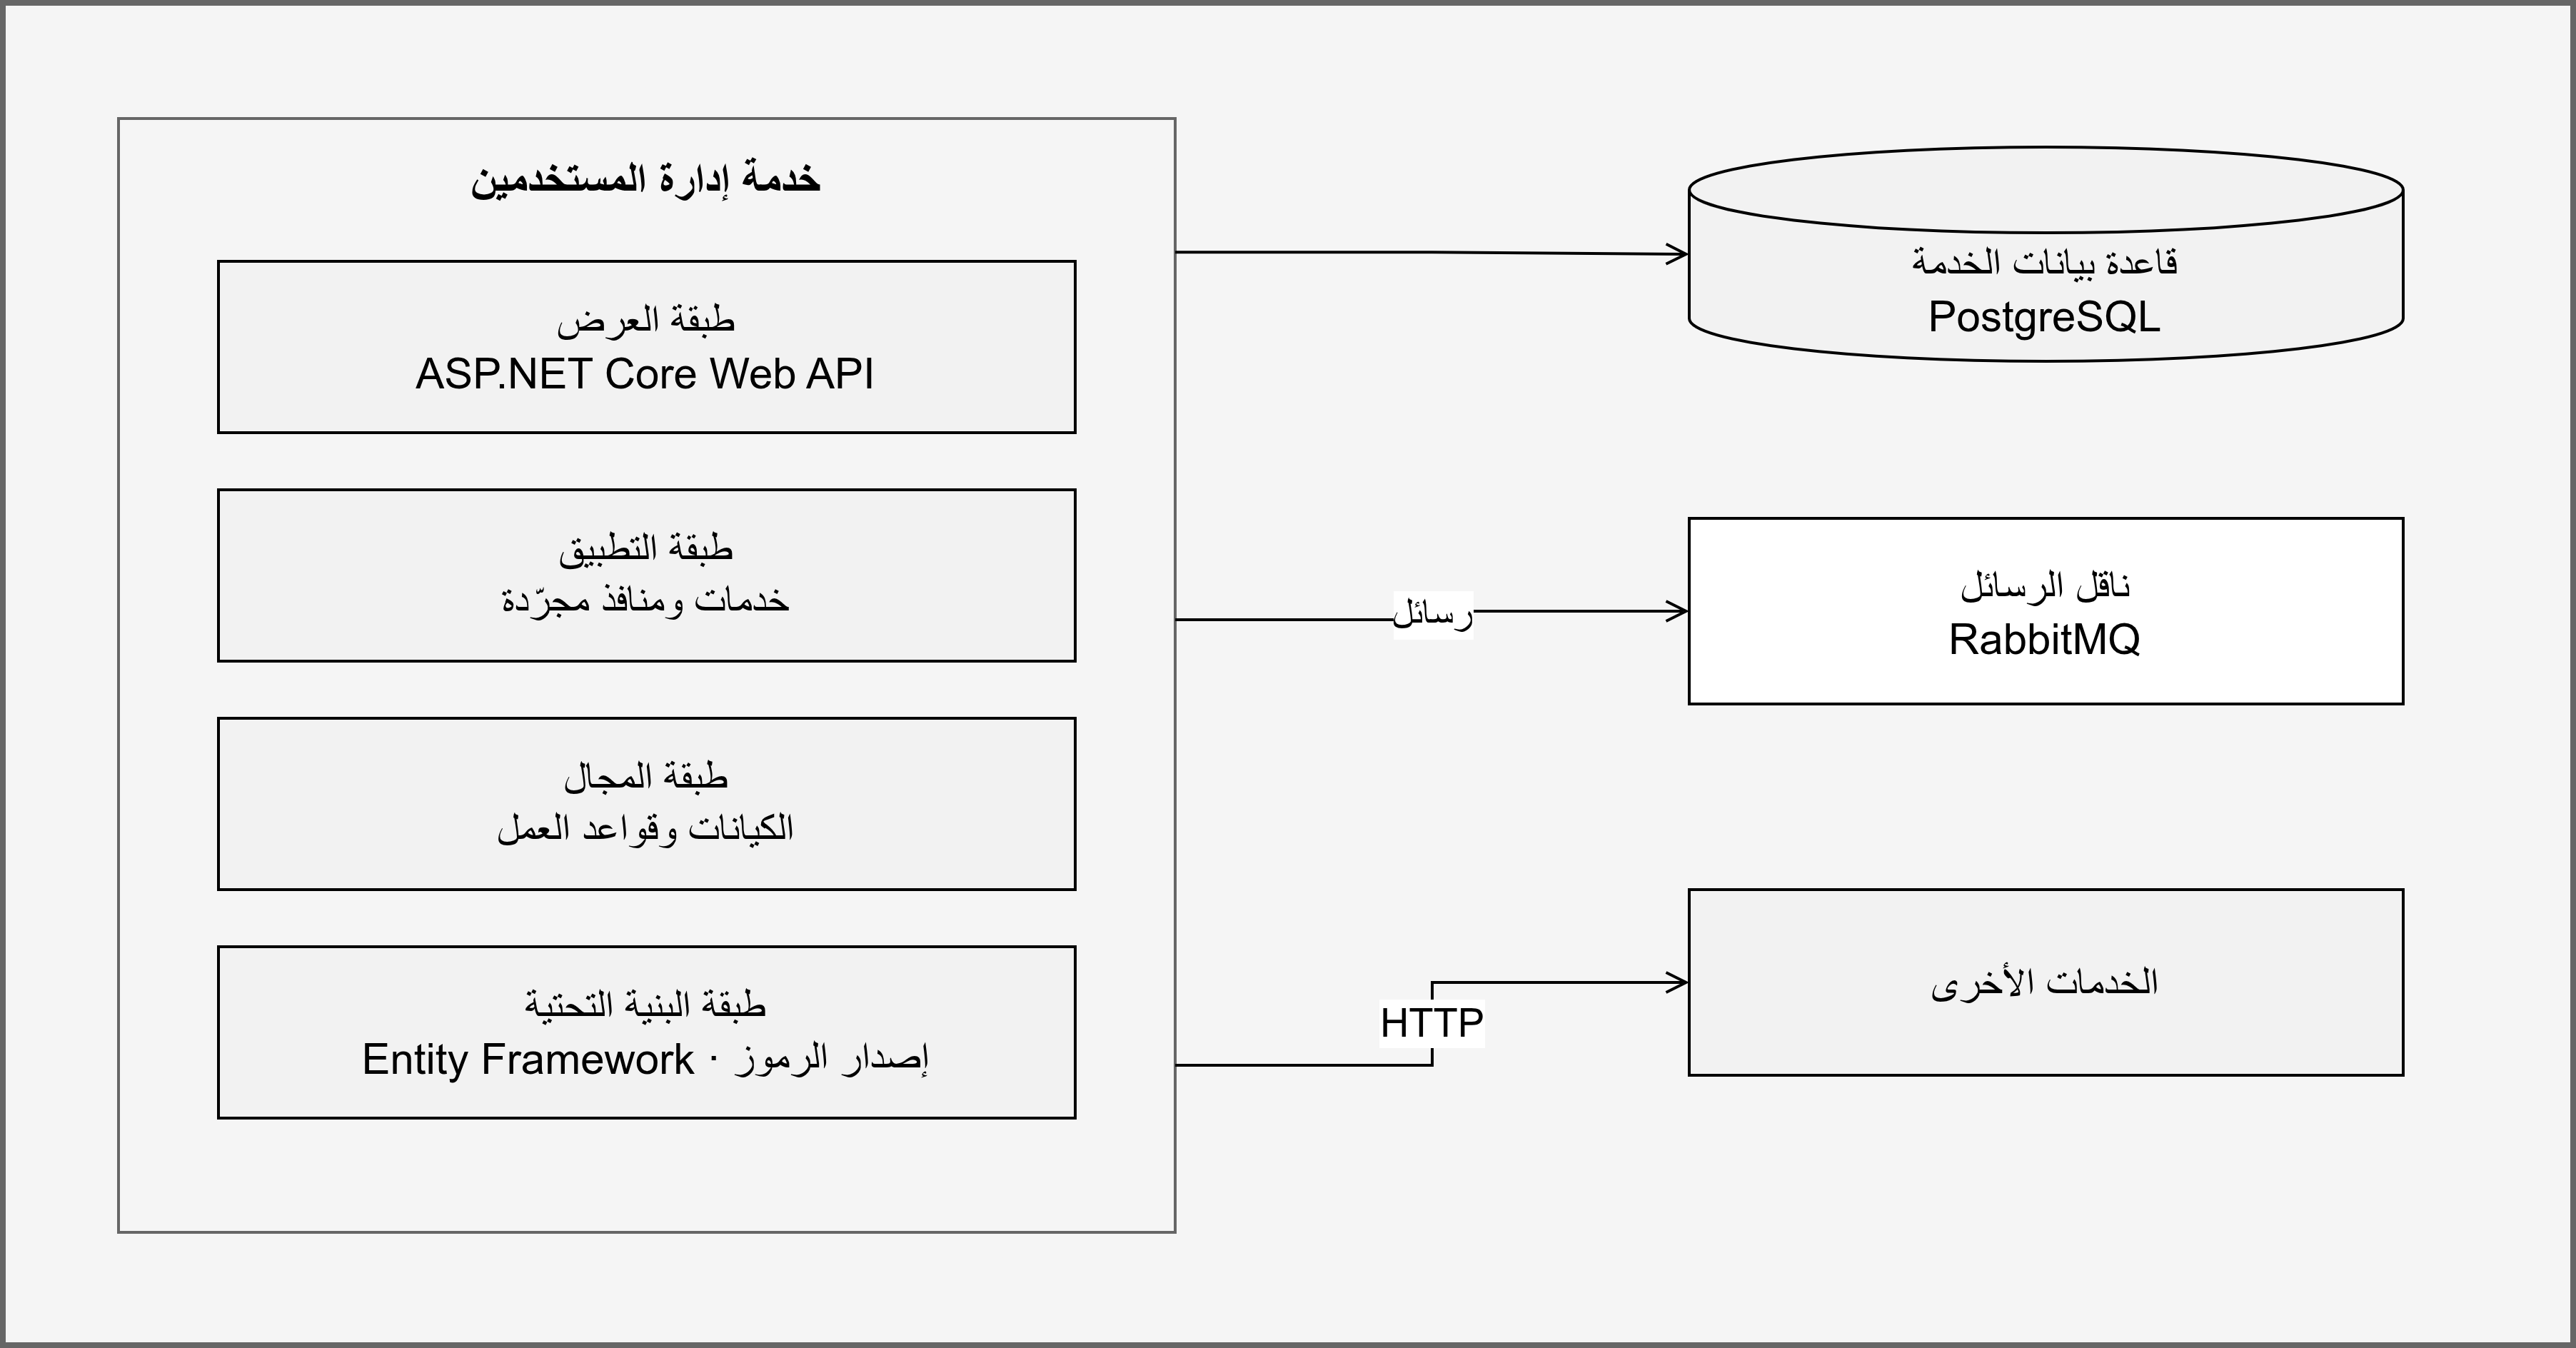
\includegraphics[width=\textwidth,height=0.8\textheight,keepaspectratio]{figures/comp-01-user-management.png}
  \caption{مخطط المكوّنات التفصيلي لخدمة إدارة المستخدمين.}
  \label{fig:comp-01}
\end{figure}

وتتّصل الخدمة بمحيطها عبر ثلاثة مسارات:

\begin{enumerate}
  \item \textbf{مولّد الرموز} (\en{JwtTokenGenerator}): تنفرد هذه الخدمة بإصدار رموز الوصول، بينما تكتفي بقية الخدمات بالتحقّق منها. ويحصر هذا التمركز أيّ تعديل على سياسة المصادقة في موضع واحد.
  \item \textbf{ناقل الإشعارات} (\en{INotificationBus}): يُستعمل لنشر ما يتطلّب تنفيذ إجراء في خدمة أخرى، كإرسال رمز العامل الثاني أو الإعلام بتغيّر حالة مستخدم.
  \item \textbf{عملاء \en{HTTP} الداخليون}: تستعملهم الواجهات الإدارية العابرة للخدمات، إذ يحتاج المدير الأعلى إلى الاطّلاع على الفصول والجلسات والمخرجات المملوكة لخدمات أخرى والتصرّف بها.
\end{enumerate}

ويُستعمل ناقل الإشعارات هنا بصيغته المباشرة، دون صندوق الصادر المعتمد في خدمة الفصول. ويقتضي نمط صندوق الصادر أن تجري الكتابة المقابلة في القاعدة نفسها وضمن المعاملة نفسها، وهو شرط لا يتحقّق حين يكون أثر الرسالة في قاعدة خدمة أخرى.

\subsection{نموذج البيانات}

يقوم نموذج بيانات الخدمة على خمسة كيانات يعرضها الشكل~\ref{fig:erd-01}: المستخدم (\en{users}) والدور (\en{roles})، ورموز التحديث (\en{refresh\_tokens})، ورموز استعادة كلمة المرور (\en{reset\_password\_tokens})، وتحدّيات العامل الثاني (\en{two\_factor\_challenges}).

\begin{figure}[htbp]
  \centering
  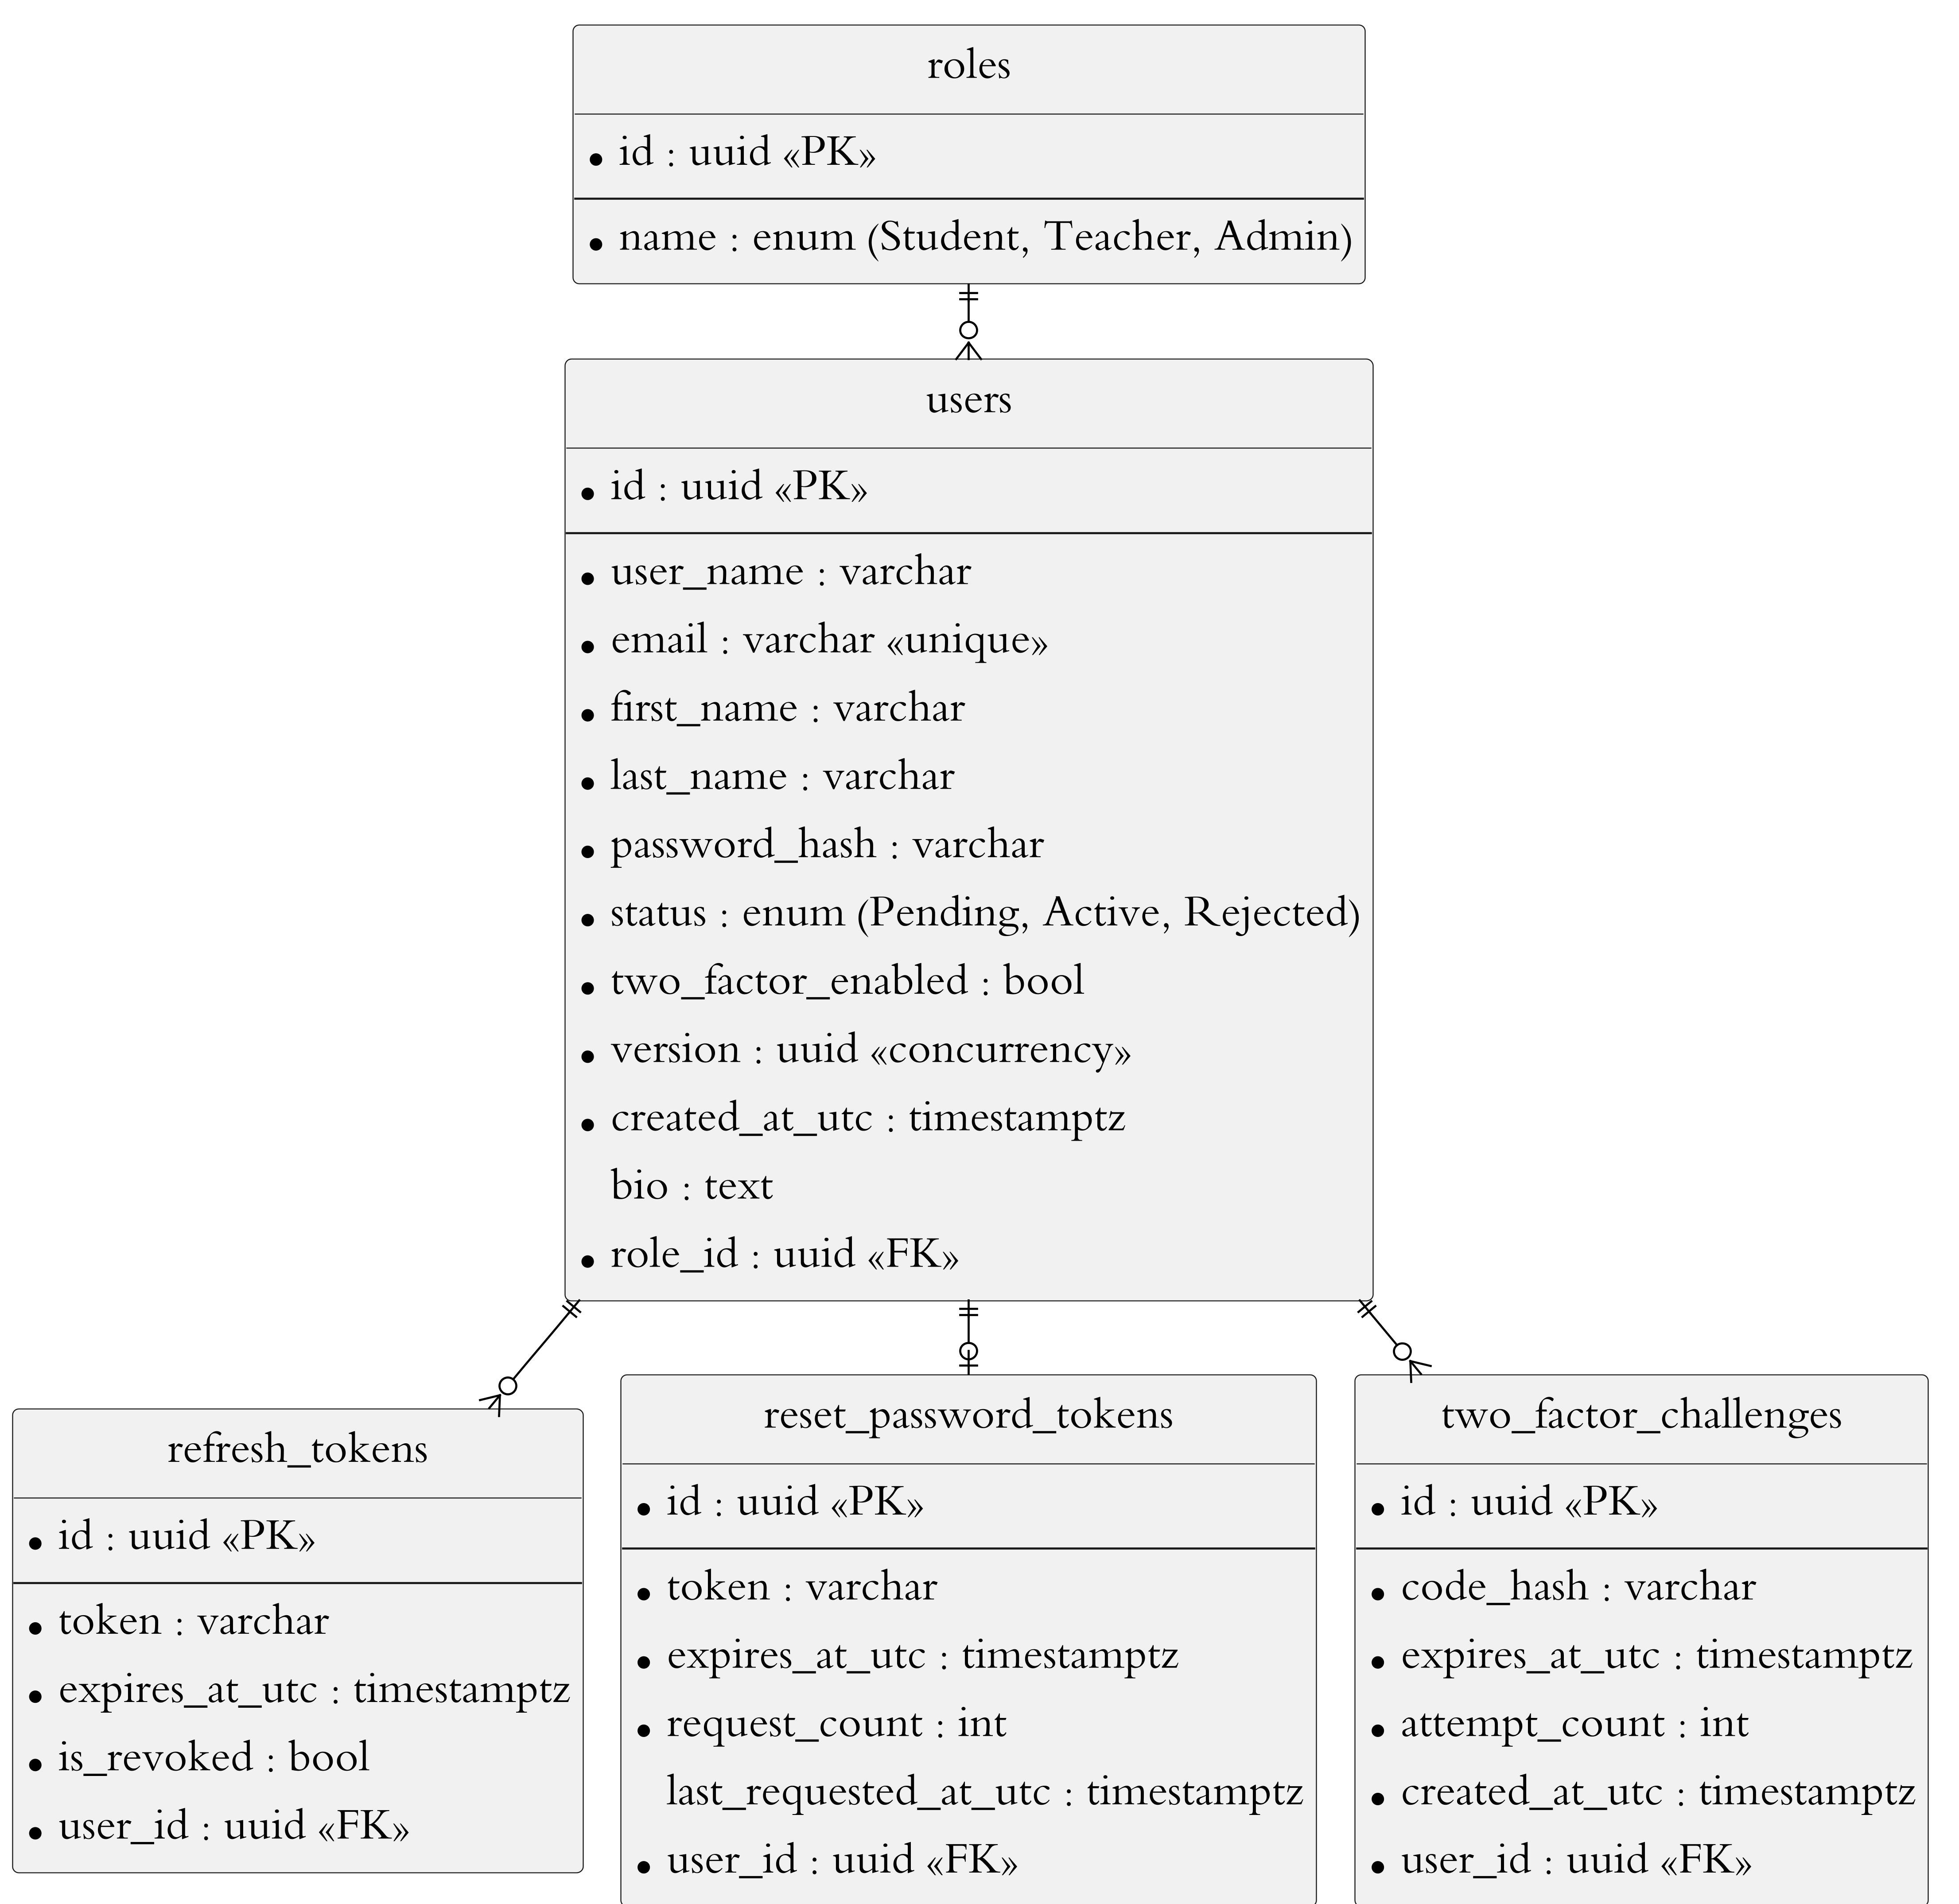
\includegraphics[width=\textwidth,height=0.8\textheight,keepaspectratio]{figures/erd-01-user-management.png}
  \caption{مخطط الكيانات والعلاقات لخدمة إدارة المستخدمين.}
  \label{fig:erd-01}
\end{figure}

وتُخزَّن الرموز الحسّاسة، وهي رمز الاستعادة ورمز العامل الثاني، على هيئة بصمات لا نصوص صريحة. ولا يمنح تسريب قاعدة البيانات عندئذٍ رمزًا صالحًا للاستعمال.

ويُبيَّن تدفّق تسجيل دخول المدير الأعلى بمرحلتيه، وما يقوم عليه من ضوابط أمنية، في القسم~\ref{subsubsec:flow-super-admin-login}.
